% 00:36 12/04/2023
\chapter{System Evaluation}
% Evaluate your project against the objectives set out in the introduction.
% This chapter should present results if applicable
% and discuss the strengths and weaknesses of your system.
% This is a clear opportunity for you to demonstrate your
% critical thinking in relation to the project.

In this chapter, I will evaluate how well the objectives were met.
I will also discuss the limitations of my platform,
including its stability and scalability.

\section{Detecting Malware}
\subsection{Dynamic Analysis}
The main goal of this project is to detect malicious software.
To achieve this, administrators can add malicious patterns through the dashboard.
These patterns are then passed to the workers when a scan task is created.
The software is executed, and its system calls are collected
and compared against the malicious patterns.
If any of the system calls contain any of the patterns,
then they can be deemed malicious.

I tested the dynamic analysis, by compiling the C program provided below
(using a compiler such as GCC or Clang).
The program creates a file called "very\_malicious.txt" when executed,
and I added this file name to the malicious patterns
before scanning the executable.

And I got the GUI application to scan this file using
the manual scan option on the main page.
\textbf{Caladium successfully detected the file as being malicious.}

\begin{lstlisting}[language=C]
#include <windows.h>

#define FILE_NAME "very_malicious.txt"

int main(int argc, char *argv[]) {
    DeleteFileA(FILE_NAME);
    CreateFile(FILE_NAME, GENERIC_WRITE, 0, NULL,
        CREATE_ALWAYS, FILE_ATTRIBUTE_NORMAL, NULL);

    return 0;
}
\end{lstlisting}

\subsection{Static Analysis}
The primary method of malware detection is dynamic analysis,
it uses static analysis as a fallback,
and uses ClamAV to facilitate this.

To test this, I am using the "EICAR Test File" \cite{EICAR},
which is a standardised file that is universally
detected as malware by all anti-malware solutions.

\textbf{Caladium successfully detected the file as malware.}

\subsection{Quarantine}
When the sandbox analysis worker detects the file as malware,
it will send a message back to the client indicating "malware\_detected".

The user in the client will then be prompted to quarantine the malware,
and the scan will finish.
\textbf{The quarantined file can be found in the quarantine frame,
concluding that the quarantining feature works correctly.}

\section{Code Quality}
I am evaluating the code quality based on its
cyclomatic complexity and its readability.

\subsection{Cyclomatic Complexity}
Cyclomatic complexity is a metric that
measures how complex code is.
This can indicate that there may be too
much code inside a class or method.

\texttt{Radon} is a tool that you can use to
calculate the code complexity of your code base. \cite{radon}

By using the \texttt{radon cc client -a} command,
I was able to measure the Python code
found in the client directory,
and it analysed the code of 48 blocks,
including classes, functions, and methods.
The average complexity for the client
was calculated as \texttt{A (2.3125)}.

I also ran the tool on the server and the average complexity
was calculated as \texttt{A (1.7567567567567568)}.
They both got grade A for complexity,
meaning the complexity is evenly distributed.

\textbf{While these are good scores for code complexity,
it does not necessarily indicate good code readability.
Readability can be improved by using good variable names.}

\subsection{Readability}
Throughout the development process,
I have made efforts to assign meaningful names
to variables that reflect their purpose.
I have also created functions to break up functionality,
which helps to keep the cyclomatic complexity low, as explained above.

In the GUI application, I have organised each frame into its own class,
such as the \texttt{QuarantineFrame},
which contains GUI-specific functionality.
The actual code for handling quarantine logic
is placed in a separate \texttt{Quarantine} class.

\textbf{I believe that following these measures has improved
the overall code readability of the application.}

\section{User Experience}
A user-friendly interface is provided to both users and
administrators through the GUI application and the dashboard.

\subsection{Windows GUI Application}
To install the software, users just need to execute the installer,
which will automatically install and provision the software,
and start it on system boot.
It will immediately begin scanning the downloads directory,
and users can easily remove the software through the preferences frame.

The quarantine frame makes it easy for users to understand which
files are quarantined and allows them to easily quarantine new files.
Users also have the ability to modify the current scanning directory.

When users scan a file, they are given real-time feedback on the scan process,
and a progress bar showing the percentage level of completion,
users can easily stop the scan process by closing the scan window.

\textbf{I believe these features, create a rich and friendly experience for users.}

\subsection{Dashboard}
Administrators are prompted to log in to the dashboard and are
given the option to change their password in the
preferences menu once logged in.

Administrators can disable dynamic analysis in case it breaks,
and the system will then solely rely on static analysis.

The dashboard is a single-page application,
which allows seamless switching between pages without loading times.
The list pages allow administrators to easily
add and remove clients or workers.

\section{RESTful APIs}
Clients communicate with the server using RESTful APIs.
Each of the endpoints is designed to be stateless,
meaning that the server does not need to maintain context.
HTTP methods such as \texttt{GET} and \texttt{POST} are used
to specify the type of action to be performed.

In the tasks endpoint, I am using the HTTP \texttt{DELETE}
method to delete records by their ID.

I have developed a suite of tests to test
the endpoints when the code is pushed to the repository.
Currently, all tests are passing. And I have also confirmed their functionality
as the GUI application is able to successfully scan files,
which relies on the APIs functioning correctly.

\textbf{GitHub shows a green check mark,
indicating all tests are passing.}

\section{Security}
As stated in the introductory chapter,
the platform needs to be secure,
it would be rather hypocritical to ignore security in a
platform targeted at identifying malware

\subsection{Authentication}
To get into the dashboard you must log in with a username and password.
The password is hashed using the SHA-256 algorithm.
If the server is compromised,
the admin's password won't be readable in its original form.

The diagram below illustrates how data can be easily
hashed, but is difficult to reverse the process.
Passwords can be securely stored after being hashed,
this makes it infeasible to retrieve the original password from the hash.

\begin{figure}[h!]
    \centering
    \label{image:hashingDiagram}
    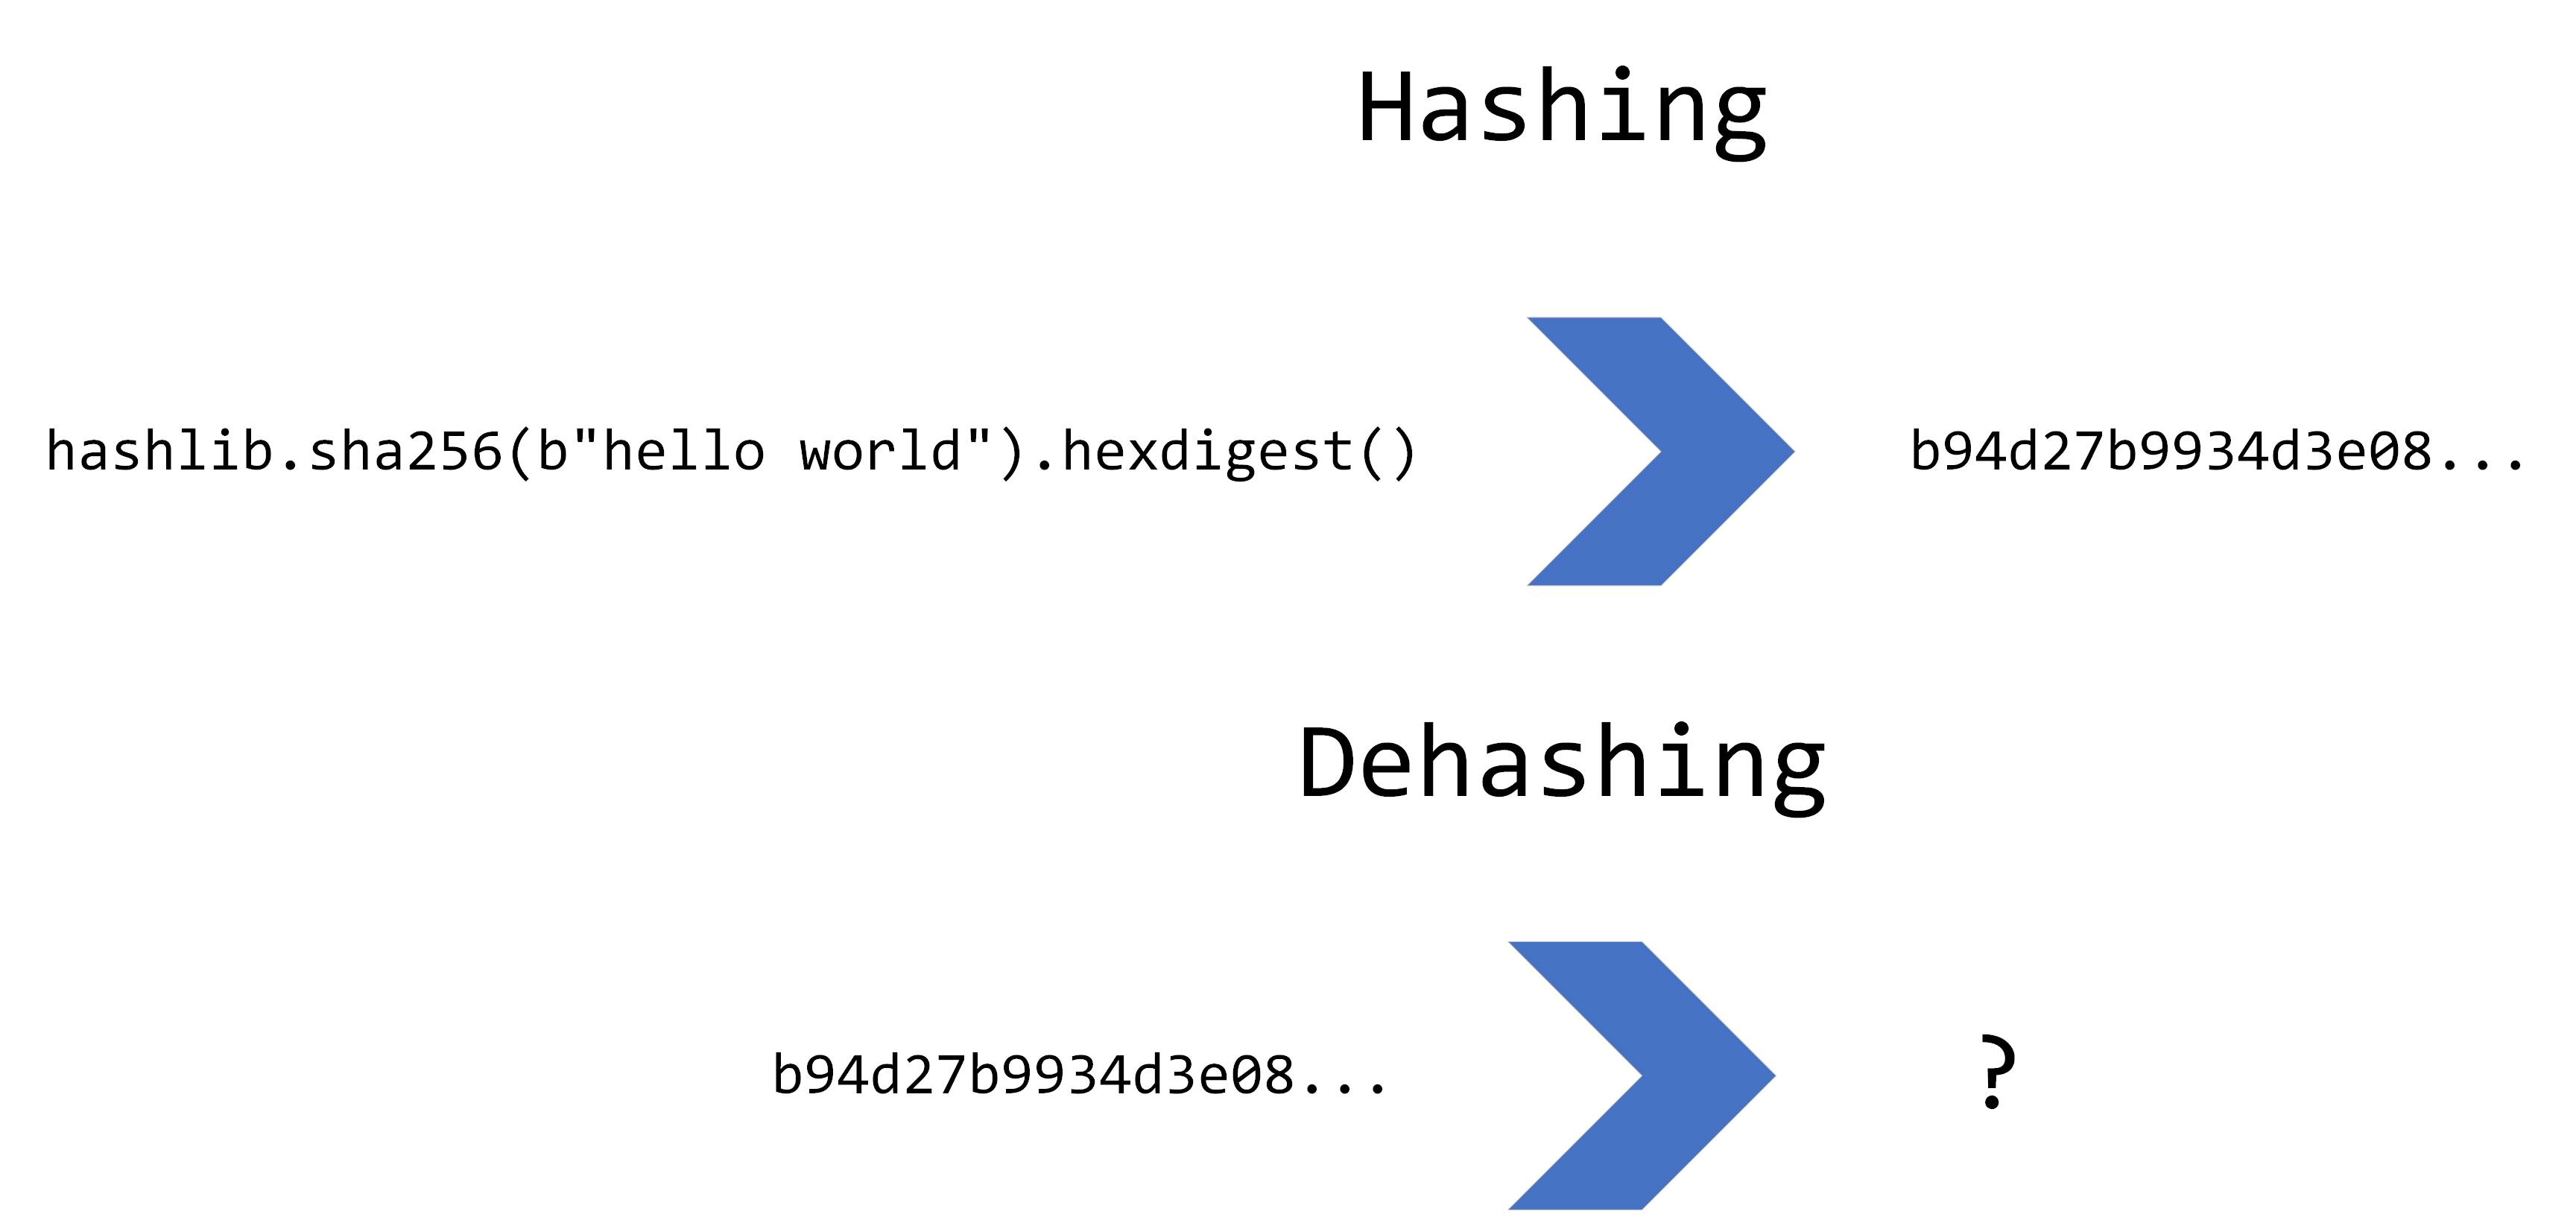
\includegraphics[width=0.75\textwidth]{images/diagrams/hashing}
    \caption{Hashing Algorithm Diagram}
\end{figure}

When you log in you are given a session token,
which is stored in the browser's local storage.
All RESTful API calls require a valid session token to be sent with the request.

In the \texttt{\_\_main\_\_.py}, you can find a function
called \texttt{before\_request},
this gets called before every request, it checks the path being requested
and if the requester has the correct token to access the resource.

\subsection{Cross Site Scripting (XSS)}
Cross-site scripting is a type of attack,
where attackers can inject code into other users' browser sessions. \cite{XSS}
A field may display data on the screen,
and attack input data may contain HTML
that is not sanitised. \\

In the screenshot below, you can see how the \\
"\texttt{hello <script>alert(1)</script>world}" string can cause a problem.
The script tags are being processed literally,
executing the JavaScript and showing the alert box.

\begin{figure}[h!]
    \centering
    \label{image:xssScreenshot}
    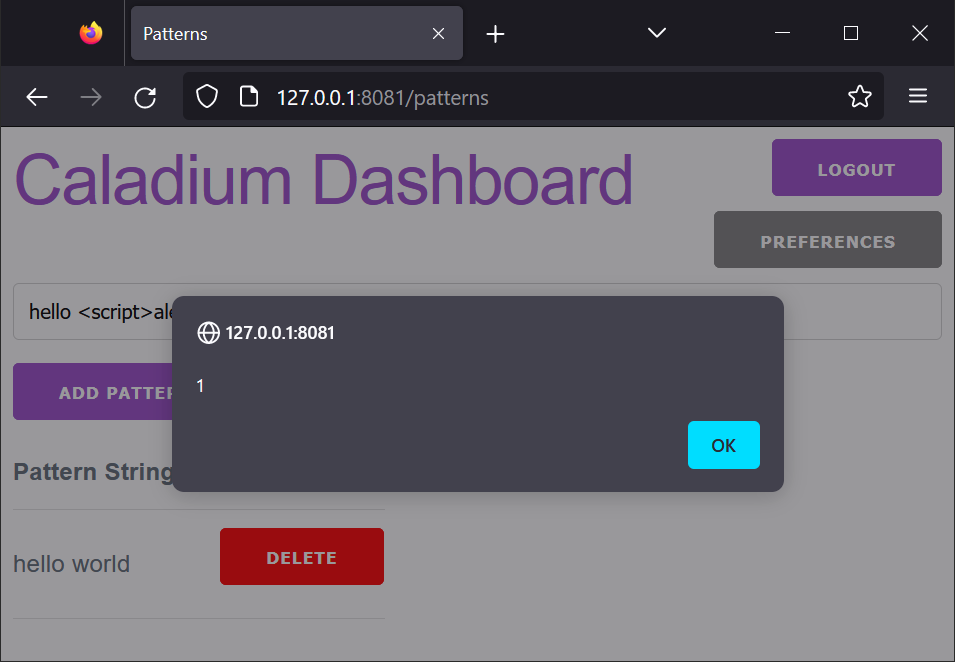
\includegraphics[width=0.85\textwidth]{images/screenshots/xss}
    \caption{Dashboard XSS Screenshot}
\end{figure}

In my project, I modified my code in the dashboard
after discovering this security bug,
to convert HTML tags to entity tags.

I added the following code, which replaces the \texttt{<}
and \texttt{>} characters with their safe equivalents.

\begin{lstlisting}
if (newHash["innerHTML"]) // Disable XSS
    newHash["innerHTML"] = newHash["innerHTML"]
    .replace('<', "&lt;").replace('>', "&gt;");
\end{lstlisting}

\section{Design Principles}
I set out from the beginning with the objective of
ensuring that the code in my project adheres to good design principles.

Throughout development, I tried to follow the
DRY (Do Not Repeat Yourself) principle as much as possible.

This is evident in the Page hierarchy found in the dashboard,
where each of the list pages shares common functionality,
this being: displaying a list of records and showing a navigation bar.
I refactored this functionality into a class called \texttt{ListPage}
that all the list pages inherit.

In the GUI application, I encapsulated the frame code into its own classes,
these classes are the ones with the \texttt{Frame} suffix,
\texttt{QuarantineFrame} for example.

\section{Stability}
Functionally, the platform works as intended,
but sometimes unexpected problems can occur
related to the networking aspect.

When designing a platform that makes use of
different languages and computers, getting everything
to work seamlessly is quite a challenge.

To try and fix this, I've added timeouts
to network requests in the GUI application when making HTTP requests.
I've also added code to catch exceptions
and present the relevant error message.

This is code from the GUI application that creates a new scan task.
Notice the timeout parameter;
this triggers an exception if it goes beyond 20 seconds.

\begin{lstlisting}
resp_obj = provisioning.caladium_api("/api/tasks", method="POST",
            data=file_data, timeout=20)
\end{lstlisting}

\section{Scaling}
The server is capable of handling multiple clients,
the platform was designed to make use of only one server,
but it is possible to have multiple instances of the server,
and have them all use the same CouchDB instance.

In the case of one server crashing,
clients using a different instance of the server
would still have the ability to scan files.

The platform can handle multiple scans at the same time,
as multiple workers are supported.

\textbf{The platform can scale by adding more analysis workers.}

\section{Time Complexity}
When a file is executed by the worker it produces a log of all the
system calls it produces, a list of patterns is passed to
the worker in order to be checked against the system calls,
if there is a match then the file can be deemed malicious.

This is a sample of the code from \texttt{sandbox/src/syscall\_analysis.py},
before optimisation it had a O($n$ * $m$) time complexity,
$n$ is the size of the syscalls
and $m$ being the size of the malicious\_patterns.

\begin{lstlisting}
def analysis_worker(syscall_queue, malicious_patterns):
  while True:
    # Fetch a syscall from the queue
    try: syscall = syscall_queue.get(timeout=1)
    except: break
    for pattern in malicious_patterns:
      # Check for a pattern match
      if pattern in syscall:
        # Detection . . .
\end{lstlisting}

Before optimisation, if the malicious\_patterns list grows
significantly this would quickly become a bottleneck,
so the solution I found is doing the checking in parallel,
each of the system calls would be added to a queue,
and a worker thread would fetch a syscall
and then compare it against all the patterns.

\textbf{This allows the analysis to quickly check all the syscalls.}

As a test, I scanned common programs that come with Microsoft Windows.
In the table below, you can find the name of the executable
and the time it took to analyse the syscalls.

\begin{table}[ht]
    \begin{tabular}{|l|c|}
        \hline
        Executable Name & Second(s) Taken to Analyse \\
        \hline
        notepad.exe & 0.84 \\
        \hline
        SnippingTool.exe & 0.89 \\
        \hline
        Defrag.exe & 1.2 \\
        \hline
    \end{tabular}
    \caption{Analysis Times}
    \label{table:analysisTimes}
\end{table}
